\documentclass[sigconf,nonacm]{acmart}

\usepackage{booktabs}
\usepackage{graphicx}
\usepackage{amsmath}
\usepackage{microtype}
\usepackage{tikz}
\usetikzlibrary{arrows.meta,positioning}
\newcommand{\showDOI}[1]{\par\noindent\textbf{DOI:} #1}
\newcommand{\fusionname}{\mbox{\textbf{\nolinkurl{siglip2_bge_bm25_fusion}}}}
\newcommand{\bestscore}[1]{\textbf{\underline{#1}}}

\acmConference[CSC1121]{CSC1121 Assignment 2}{2026}{Dublin City University}
\acmBooktitle{CSC1121 Assignment 2 (CSC1121), 2026, Dublin City University}
\settopmatter{printacmref=false}

\begin{document}
\raggedbottom
\setlength{\textfloatsep}{10pt plus 2pt minus 2pt}
\setlength{\floatsep}{8pt plus 2pt minus 2pt}
\setlength{\intextsep}{8pt plus 2pt minus 2pt}

\title{Multimodal Object Search over Egocentric Lifelogging Video: The CASTLE 2024 Dataset}

\author{Arun Narayanan}
\email{arun.narayanan2@mail.dcu.ie}
\affiliation{
  \institution{Dublin City University}
  \department{School of Computing}
  \city{Dublin}
  \country{Ireland}
}

\begin{abstract}
We present a multimodal information retrieval system for the CASTLE 2024 egocentric lifelogging dataset, comprising 416,542 keyframes sampled at 5-second intervals across four recording days and fifteen camera streams. Three retrieval approaches are implemented and evaluated. Approach A is a sparse BM25 baseline over ASR transcripts and \textbf{Florence-2} visual captions. Approach B performs dense visual retrieval with \textbf{SigLIP2} SO400M embeddings over the full frame corpus. Approach C, the primary contribution, combines sparse text, dense text, and dense visual signals through weighted late fusion, then applies cross-encoder reranking with \textbf{bge-reranker-v2-m3} over the top-50 candidates. Evaluation on 10 queries against 71 manually judged relevant frames yields mean Precision@10 scores of 0.070, 0.620, and 0.640 for Approaches A, B, and C respectively. The results show that dense visual retrieval is the strongest signal for this task, while fusion provides the best overall effectiveness. As an indexing contribution, we introduce an OCR hallucination gate that uses \textbf{SigLIP2} cosine similarity to remove 178,914 ungrounded OCR-bearing caption records before retrieval. An interactive Streamlit interface supports query selection, approach switching, and Rocchio relevance feedback for iterative refinement.

\end{abstract}

\keywords{egocentric video retrieval, multimodal IR, SigLIP2, late fusion, lifelogging, CASTLE 2024, BM25, cross-encoder re-ranking}

\maketitle
\begingroup
\renewcommand{\thefootnote}{}
\footnotetext{GitHub Repository: \url{https://github.com/ArunGMR0411/ir-text2Image}}
\endgroup

\section{Introduction}
\label{sec:introduction}

Multimodal retrieval over egocentric video presents challenges unlike those in web image search or broadcast video retrieval. In lifelogging corpora, activities are observed from a first-person perspective, queried objects may be small or partially occluded, and speech transcripts are generated by automatic speech recognition systems that do not always align with the visual evidence available in a single frame. As a result, sparse keyword matching alone is often insufficient, particularly for visually grounded queries where the relevant signal is weak or absent in the transcript stream. These characteristics motivate retrieval architectures that treat dense visual representations as a primary signal rather than as a secondary reranking feature \cite{gurrin2024castle}.

The CASTLE 2024 dataset provides a realistic testbed for studying this problem. It contains 416,542 keyframes sampled at 5-second intervals across four recording days, spanning ten egocentric member cameras and five fixed room cameras: kitchen, living1, living2, meeting, and reading. Each frame follows the \textbf{HH\_NNNN.webp} naming convention, where \textbf{HH} denotes the hour of day and \textbf{NNNN} is a four-digit frame counter within that hour. Machine-generated ASR transcripts are aligned to frames using a 20-second sliding window, producing 145,140 transcript-frame pairs that supply conversational context when it is available.

Our system is organised as a three-stage pipeline consisting of feature extraction, multi-index retrieval, and final ranking. Approach A uses BM25 as a sparse text baseline over transcripts and \textbf{Florence-2} machine-generated visual captions, explicitly satisfying the assignment requirement for an inverted index while providing a transparent lexical baseline \cite{robertson2009probabilistic}. Approach B uses \textbf{SigLIP2} SO400M embeddings as the dense visual retrieval backbone, leveraging the strong cross-modal alignment induced by sigmoid-loss pre-training \cite{zhai2023sigmoid}. Approach C is the principal contribution. It combines BM25 scores, \textbf{BGE-large-en-v1.5} dense text embeddings, and \textbf{SigLIP2} visual embeddings through weighted late fusion, then applies cross-encoder reranking with the \textbf{bge-reranker-v2-m3} model over the top-50 candidates. This design allows the system to exploit complementary evidence from sparse lexical matching, dense semantic text retrieval, and dense visual similarity, while still preserving a controllable ranking pipeline \cite{chen2024bge}. Figure~\ref{fig:architecture} illustrates the seven-layer system architecture.

\begin{figure}[t]
  \centering
  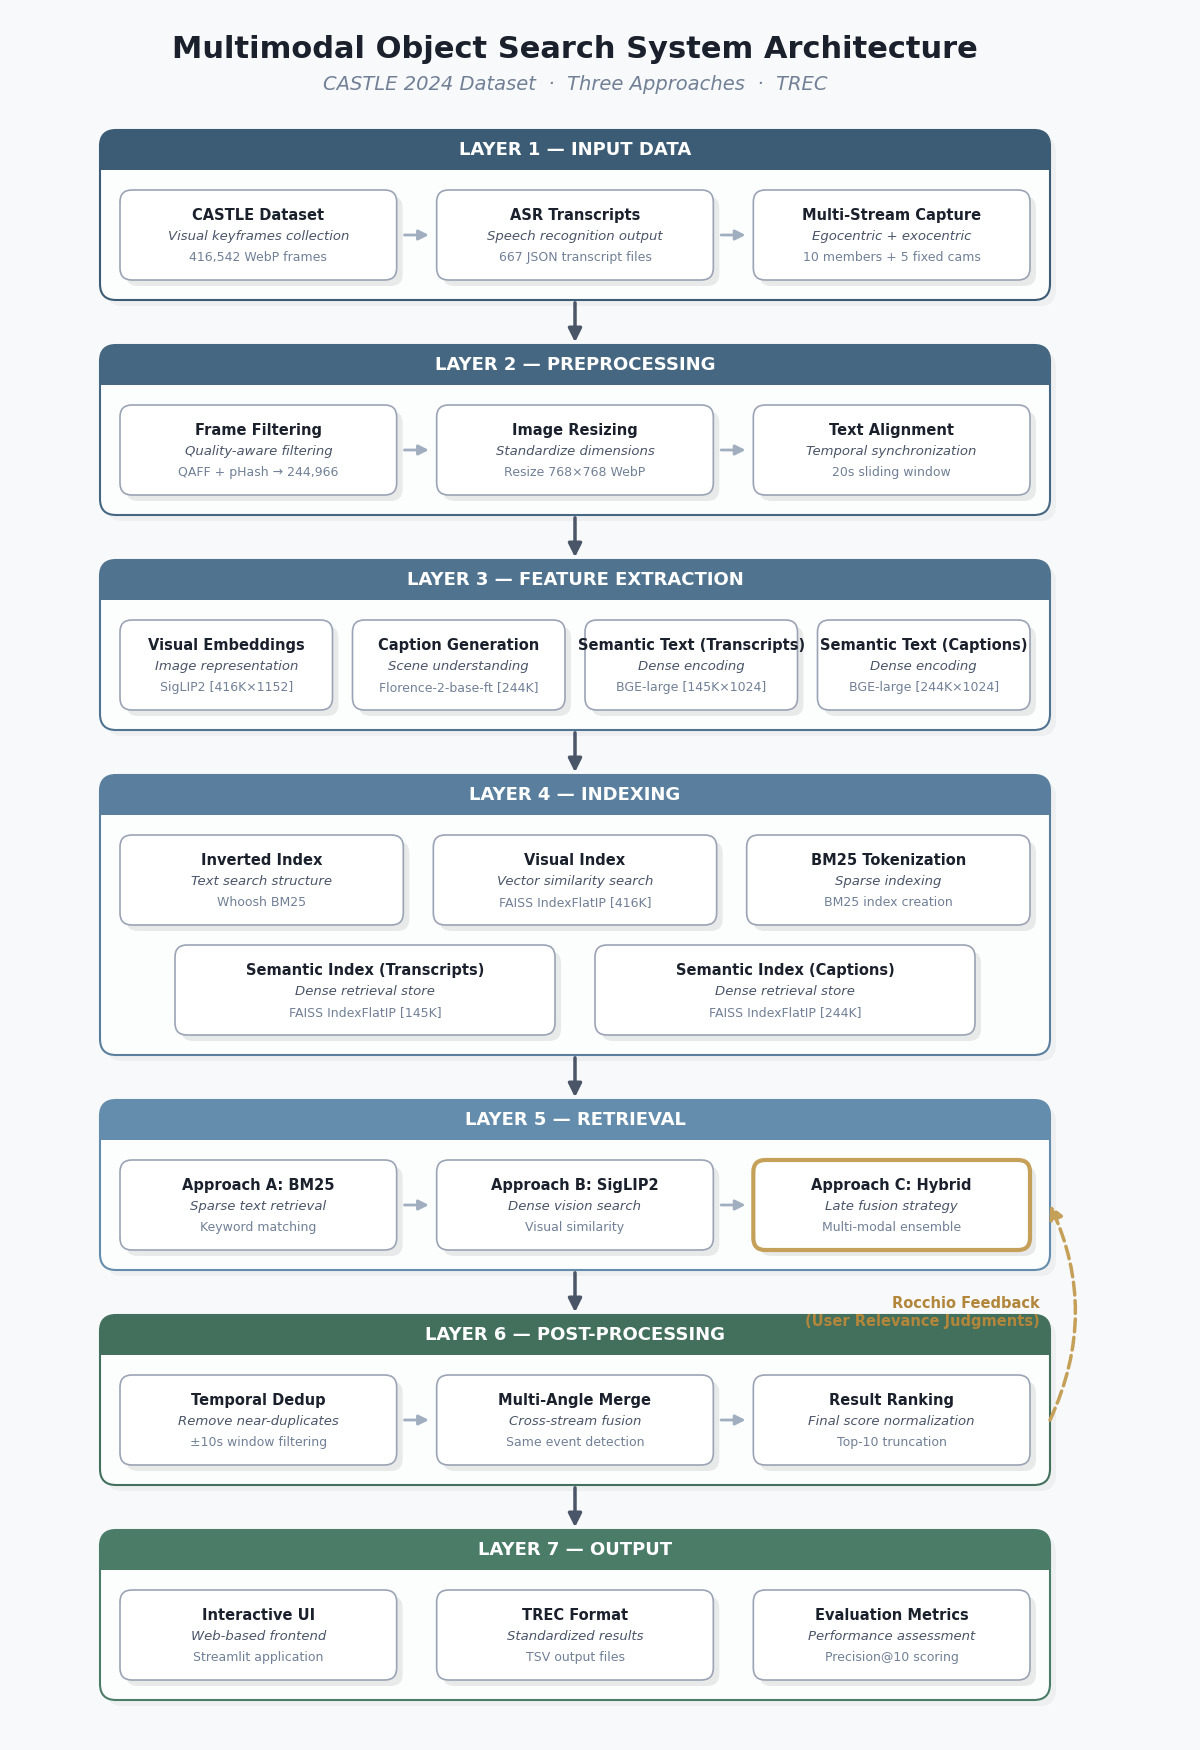
\includegraphics[width=\linewidth]{figures/architecture_diagram_v2}
  \caption{System architecture of the MOS pipeline. Seven layers cover input data, preprocessing, feature extraction, indexing, retrieval, post-processing, and output.}
  \label{fig:architecture}
  \Description{Seven-layer system diagram showing data input, preprocessing, feature extraction, indexing, retrieval, post-processing, and output stages in the MOS pipeline.}
\end{figure}

To support interactive exploration, we also provide a Streamlit interface with query selection, approach switching, result inspection, and Rocchio-style relevance feedback driven by \textbf{SigLIP2} vector blending \cite{rocchio1971relevance}. The remainder of the paper is structured as follows. Section~\ref{sec:indexing} describes the indexing pipeline, including the OCR hallucination gate. Section~\ref{sec:ranking} details the three retrieval approaches and post-processing stages. Section~\ref{sec:evaluation} presents the Precision@10 evaluation and analysis. Section~\ref{sec:conclusions} concludes the paper and outlines future work.

\section{Indexing}
\label{sec:indexing}

The indexing pipeline transforms the CASTLE 2024 corpus into a unified multimodal retrieval substrate through dataset preparation, visual feature extraction, text feature extraction, OCR hallucination mitigation, and multi-index construction. The design goal is to retain exact frame-level correspondence across modalities while controlling storage, redundancy, and noise.

Figure~\ref{fig:indexing-flow} summarises the indexing workflow from raw keyframes to the final set of retrieval artifacts.

\begin{figure}[t]
  \centering
  \resizebox{0.94\linewidth}{!}{%
  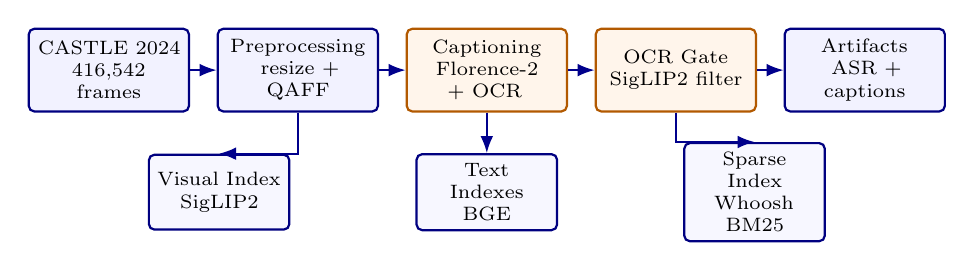
\begin{tikzpicture}[
    x=1cm, y=1cm,
    >=Latex,
    node distance=0.25cm,
    stage/.style={
      draw=blue!50!black,
      rounded corners=2pt,
      thick,
      fill=blue!5,
      align=center,
      text width=1.8cm,
      minimum height=1.05cm,
      font=\scriptsize
    },
    accent/.style={
      stage,
      draw=orange!70!black,
      fill=orange!8
    },
    outbox/.style={
      draw=blue!50!black,
      rounded corners=2pt,
      thick,
      fill=blue!3,
      align=center,
      text width=1.55cm,
      minimum height=0.95cm,
      font=\scriptsize
    },
    flow/.style={->, line width=0.7pt, draw=blue!55!black}
  ]
    \node[stage] (castle) at (0.6,1.55) {CASTLE 2024\\416,542 frames};
    \node[stage] (prep) at (3.0,1.55) {Preprocessing\\resize + QAFF};
    \node[accent] (caption) at (5.4,1.55) {Captioning\\Florence-2 + OCR};
    \node[accent] (gate) at (7.8,1.55) {OCR Gate\\SigLIP2 filter};
    \node[stage] (artifacts) at (10.2,1.55) {Artifacts\\ASR + captions};

    \node[outbox] (visual) at (2.0,0.0) {Visual Index\\SigLIP2};
    \node[outbox] (text) at (5.4,0.0) {Text Indexes\\BGE};
    \node[outbox] (sparse) at (8.8,0.0) {Sparse Index\\Whoosh BM25};

    \draw[flow] (castle) -- (prep);
    \draw[flow] (prep) -- (caption);
    \draw[flow] (caption) -- (gate);
    \draw[flow] (gate) -- (artifacts);

    \draw[flow] (prep.south) |- (visual.north);
    \draw[flow] (caption.south) -- (text.north);
    \draw[flow] (gate.south) |- (sparse.north);
  \end{tikzpicture}
  }
  \caption{Indexing workflow from raw CASTLE 2024 keyframes through preprocessing, caption cleaning, and multi-index construction.}
  \label{fig:indexing-flow}
  \Description{Flowchart showing the indexing pipeline: CASTLE 2024 keyframes, preprocessing and frame filtering, Florence-2 caption generation, OCR gating, and the final visual, semantic, and sparse indexes.}
\end{figure}

\subsection{Dataset and Keyframe Corpus}
\label{sec:dataset}

The CASTLE 2024 dataset spans four recording days and combines ten egocentric member cameras with five fixed room cameras, yielding 416,542 keyframes sampled at 5-second intervals. The fixed streams correspond to kitchen, living1, living2, meeting, and reading. Each keyframe follows the \textbf{HH\_NNNN.webp} naming convention, where the hour token identifies the source hour and the four-digit counter identifies the frame position within that hour. Temporal alignment uses the verified offset rule
\[
  t_{\text{offset}} = (\text{NNNN} - 1) \times 5
\]
which was validated against transcript timing across multiple streams and days.

The raw 4K UHD corpus was resized to 768$\times$768 using \textbf{cv2.INTER\_LANCZOS4} and stored as WebP with quality 90, reducing storage from 107.61 GB to 41.28 GB. To reduce the cost of downstream caption generation, we applied a two-stage Quality-Aware Frame Filtering (QAFF) procedure. First, CLIP ViT-B/32 query-aware relevance scores were computed for all 416,542 frames. The resulting distribution was tightly compressed, with minimum 0.1612, maximum 0.3397, mean 0.2311, and median 0.2288. Histogram inspection motivated three score tiers: HOT for scores at least 0.27, WARM for scores from 0.20 to 0.27, and COLD for scores below 0.20, producing 29,011 HOT frames, 354,512 WARM frames, and 33,019 COLD frames. A perceptual-hash decimation stage then filtered WARM and COLD frames using Hamming-distance thresholds of 8 and 12 respectively, while preserving all HOT frames. The final captioning subset contained 244,966 frames, meaning 171,576 frames were removed. Fixed cameras showed a 78.4\% drop rate compared with 1.2\% for member cameras, which is consistent with the stronger redundancy in room-mounted views, and the main corpus statistics are summarised in Table~\ref{tab:dataset-stats}.

\begin{table}[t]
\centering
\small
\resizebox{\columnwidth}{!}{%
\begin{tabular}{ll}
\toprule
Metric & Value \\
\midrule
Total keyframes & 416542 \\
Recording days & 4 \\
Member streams (egocentric) & 10 \\
Fixed room cameras & 5 \\
Total streams & 60 \\
Frame sampling interval & 5.0 seconds \\
Frames after pHash decimation (captioning corpus) & 244966 \\
Frames dropped by pHash & 171576 \\
HOT frame preservation rate & 100\% \\
Fixed camera drop rate & 78.4\% \\
Member camera drop rate & 1.2\% \\
Transcript JSON files & 667 \\
Transcript-aligned frame pairs & 145140 \\
Original dataset size & 107.61 GB \\
Resized dataset size (768x768 WebP) & 41.28 GB \\
\bottomrule
\end{tabular}
}
\caption{CASTLE 2024 dataset and preprocessing statistics.}
\label{tab:dataset-stats}
\end{table}

\subsection{Visual Feature Extraction}
\label{sec:visual-features}

Dense visual representations were extracted with \textbf{SigLIP2} SO400M. This model was preferred because sigmoid-loss pre-training yields strong cross-modal alignment for fine-grained object-centric retrieval \cite{zhai2023sigmoid}. The final float32 embedding matrix has shape 416,542$\times$1,152 and occupies approximately 1.79 GB on disk.

\subsection{Text Feature Extraction}
\label{sec:text-features}

ASR transcripts were aligned to keyframes with a 20-second sliding window, that is, \(\pm 10\) seconds around the current chunk start time, producing 145,140 transcript-frame pairs from 667 transcript JSON files. Transcript cleaning applied lowercasing, punctuation removal, tokenisation, and stopword filtering, reducing average transcript length from 122.02 words to 69.76 words per frame.

Dense semantic text features were generated with \textbf{BGE-large-en-v1.5} \cite{chen2024bge}. The transcript embedding matrix has shape 145,140$\times$1,024 and occupies approximately 0.55 GiB, while the caption embedding matrix has shape 244,966$\times$1,024 and occupies approximately 0.93 GiB. Visual captions were generated with \textbf{Florence-2} \cite{xiao2023florence2} using a two-pass design that applied both caption and OCR prompts per frame. The pipeline produced 244,966 caption records covering the decimated keyframe corpus.

\subsection{OCR Hallucination Gate}
\label{sec:ocr-gate}

Inspection of the caption corpus showed that \textbf{Florence-2} frequently appended OCR-bearing strings to frames that contained no visually grounded writing. In total, 178,914 records exhibited this behaviour. To suppress this noise without a second visual inference pass, each OCR string was encoded with the \textbf{SigLIP2} text tower and compared against the corresponding 1,152-dimensional visual embedding using cosine similarity. OCR-bearing text was stripped whenever similarity fell below 0.20.

This gate removed all 178,914 affected records, yielding a 100\% strip rate. Observed similarities ranged from -0.081 to 0.137, with mean 0.043, well below the threshold. The outcome is consistent with the learned sigmoid parameters of \textbf{SigLIP2}: the approximate logit scale is 4.70 and the bias is -15.93, implying a breakeven cosine of roughly 3.39, which is impossible for unit-normalised vectors. In practical terms, the gate prevents OCR hallucinations from polluting both the sparse \textbf{Whoosh} index and the dense caption embedding space, as detailed in Table~\ref{tab:ocr-gate}.

\begin{table}[t]
\centering
\small
\resizebox{\columnwidth}{!}{%
\begin{tabular}{ll}
\toprule
Metric & Value \\
\midrule
Total caption records & 244966 \\
Records with non-empty OCR text & 178914 \\
OCR records stripped (hallucinated) & 178914 \\
Strip rate & 100.0\% \\
Records retained (sim >= 0.20) & 0 \\
Cosine similarity minimum & -0.081 \\
Cosine similarity mean & 0.043 \\
Cosine similarity maximum & 0.137 \\
Gate threshold & 0.20 \\
SigLIP2 logit scale & \textasciitilde4.70 \\
SigLIP2 logit bias & \textasciitilde-15.93 \\
Breakeven cosine for sigmoid=0.5 & \textasciitilde3.39 (impossible for unit vectors) \\
Captions under 5 words (post-gate artefacts) & 1639 \\
True in-body hallucination rate & 0.0024\% (6 records) \\
\bottomrule
\end{tabular}
}
\caption{OCR hallucination gate statistics. All 178,914 ungrounded tokens were stripped at a 100\% rate.}
\label{tab:ocr-gate}
\end{table}

\subsection{Index Architecture}
\label{sec:index-arch}

The final retrieval architecture uses three modality-specific indexes. The visual index stores 416,542 \textbf{SigLIP2} vectors in a \textbf{FAISS IndexFlatIP} structure for exact cosine retrieval \cite{johnson2021billion}. Two additional \textbf{FAISS IndexFlatIP} indexes store transcript and caption embeddings, with sizes of approximately 0.55 GiB and 0.93 GiB respectively. Sparse lexical retrieval is handled by a \textbf{Whoosh BM25} index spanning seven fields: \textbf{frame\_id}, \textbf{stream\_name}, \textbf{day}, \textbf{hour}, \textbf{timestamp\_str}, \textbf{transcript\_text}, and \textbf{caption\_text}, and the resulting multi-index design is summarised in Table~\ref{tab:index-arch}.

Flat indexing was selected because the corpus fits comfortably in main memory without requiring quantisation. This preserves exact retrieval fidelity across visual and textual modalities while keeping the architecture simple, deterministic, and easy to analyse.

\begin{table}[t]
\centering
\small
\resizebox{\columnwidth}{!}{%
\begin{tabular}{llllll}
\toprule
Index Name & Type & Dimension & Vectors & File Size & Notes \\
\midrule
Visual Index & \textbf{FAISS IndexFlatIP} & 1152 & 416542 & 1.79 GiB & SigLIP2 embeddings --- exact cosine search \\
Transcript Semantic Index & \textbf{FAISS IndexFlatIP} & 1024 & 145140 & 0.55 GiB & BGE-large-en-v1.5 embeddings \\
Caption Semantic Index & \textbf{FAISS IndexFlatIP} & 1024 & 244966 & 0.93 GiB & BGE-large-en-v1.5 embeddings \\
Sparse Keyword Index & \textbf{Whoosh BM25} & --- & 416542 & --- & 7 retrieval fields \\
\bottomrule
\end{tabular}
}
\caption{Multi-index architecture of the MOS retrieval system.}
\label{tab:index-arch}
\end{table}

\section{Ranking and Retrieval Methodology}
\label{sec:ranking}

The retrieval system implements three approaches that are evaluated both individually and as components of a unified multimodal ranking pipeline. As summarised in Table~\ref{tab:approach-overview}, the approaches differ in signal type, index structure, and ranking strategy, while sharing common post-processing operations before final top-10 output.

Figure~\ref{fig:retrieval-flow} provides a compact view of how the three approaches feed into the shared ranking and output stage.

\begin{figure}[t]
  \centering
  \resizebox{0.94\linewidth}{!}{%
  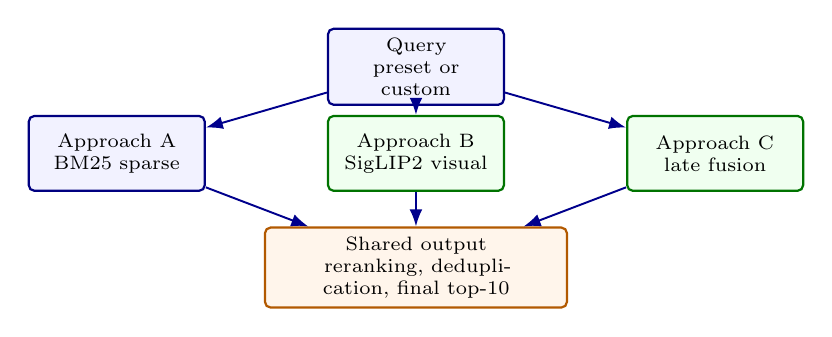
\begin{tikzpicture}[
    x=1cm, y=1cm,
    >=Latex,
    stage/.style={
      draw=blue!50!black,
      rounded corners=2pt,
      thick,
      fill=blue!5,
      align=center,
      text width=2.0cm,
      minimum height=0.95cm,
      font=\scriptsize
    },
    accent/.style={
      stage,
      fill=green!6,
      draw=green!45!black
    },
    final/.style={
      stage,
      fill=orange!8,
      draw=orange!70!black,
      text width=3.6cm
    },
    flow/.style={->, line width=0.7pt, draw=blue!55!black}
  ]
    \node[stage] (query) at (5.4,2.0) {Query\\preset or custom};
    \node[stage] (a) at (1.6,0.9) {Approach A\\BM25 sparse};
    \node[accent] (b) at (5.4,0.9) {Approach B\\SigLIP2 visual};
    \node[accent] (c) at (9.2,0.9) {Approach C\\late fusion};
    \node[final] (out) at (5.4,-0.55) {Shared output\\reranking, deduplication, final top-10};

    \draw[flow] (query) -- (a);
    \draw[flow] (query) -- (b);
    \draw[flow] (query) -- (c);
    \draw[flow] (a) -- (out);
    \draw[flow] (b) -- (out);
    \draw[flow] (c) -- (out);
  \end{tikzpicture}
  }
  \caption{Retrieval and ranking workflow across Approaches A, B, and C, ending in shared post-processing and final top-10 output.}
  \label{fig:retrieval-flow}
  \Description{Flowchart showing a query entering three retrieval branches: BM25 sparse retrieval, SigLIP2 visual retrieval, and late fusion retrieval, which then feed into shared reranking, deduplication, and final top-10 results.}
\end{figure}

\subsection{Approach A: Sparse Text Retrieval}
\label{sec:approach-a}

\begin{table}[t]
\small
\centering
\caption{Overview of the three retrieval approaches.}
\label{tab:approach-overview}
\resizebox{\columnwidth}{!}{%
\begin{tabular}{llll}
\toprule
Property & Approach A & Approach B & Approach C \\
\midrule
Full Name & BM25 Sparse Text Retrieval & SigLIP2 Dense Visual Retrieval & Hybrid Late Fusion with Cross-Encoder Re-ranking \\
Type & Sparse Inverted Index & Dense Vector Retrieval & Hybrid Late Fusion \\
Visual Signal & Florence-2 Captions & SigLIP2 Embeddings & SigLIP2 Embeddings \\
Text Signal & Transcripts + Captions & None & Transcripts + Captions \\
Semantic Signal & None & SigLIP2 Cross-modal & BGE-large-en-v1.5 \\
Re-ranking & None & None & bge-reranker-v2-m3 (top-50 candidates) \\
Index & Whoosh BM25 & FAISS IndexFlatIP & BM25 + FAISS$\times$3 \\
Mean P@10 & 0.070 & 0.620 & 0.640 \\
Role & Sparse Baseline & Dense Visual Baseline & Primary Novel Submission \\
\bottomrule
\end{tabular}
}
\end{table}

Approach A is a sparse inverted-index retrieval system built on \textbf{Whoosh BM25} over two text streams: ASR transcripts and \textbf{Florence-2} visual captions. This branch explicitly fulfils the assignment requirement for an inverted index. Each keyframe is represented as a text document containing transcript evidence from the 20-second alignment window together with the corresponding visual caption. At query time, the natural-language query is tokenised and scored using Okapi BM25 \cite{robertson2009probabilistic}.

To mitigate vocabulary mismatch, the query-expansion stage augments the user query with synonyms, object hints, and colour hints. These terms are combined with a disjunctive query formulation, which proved more robust than conjunction-based matching for multi-term lifelogging queries. A location-aware post-filter then reduces location-mismatched results by 50\% whenever the frame stream is incompatible with the query location prior. All resulting scores are max-normalised into the range $[0,1]$ before any downstream fusion.

\subsection{Approach B: Dense Visual Retrieval}
\label{sec:approach-b}

Approach B performs dense retrieval exclusively in the visual embedding space. Every keyframe is encoded with \textbf{SigLIP2} into a 1,152-dimensional representation, and every natural-language query is projected into the same space using the paired text encoder. Retrieval is then carried out by maximum inner-product search over the full \textbf{FAISS} visual index, implemented as \textbf{IndexFlatIP} \cite{johnson2021billion}. Because vectors are normalised before retrieval, inner-product search is equivalent to cosine similarity.

\textbf{SigLIP2} was selected over standard CLIP baselines because its sigmoid-loss formulation yields stronger cross-modal alignment for fine-grained object and scene retrieval \cite{zhai2023sigmoid}. This visual-only pathway is particularly important for object-centric queries, where transcript evidence is often absent or too noisy to discriminate relevant frames.

\subsection{Approach C: Hybrid Late Fusion with Cross-Encoder Re-ranking}
\label{sec:approach-c}

Approach C, labelled \fusionname, is the primary contribution of the system. It combines three independently generated candidate signals: visual scores from \textbf{SigLIP2}, dense semantic text scores from \textbf{BGE-large-en-v1.5} over transcripts and captions \cite{chen2024bge}, and sparse BM25 scores from Approach A. Per-query fusion weights are listed in Table~\ref{tab:fusion-weights}.

\begin{table*}[!t]
\small
\centering
\caption{Per-query late fusion weights for \fusionname. $w_{\text{vis}}$ and $w_{\text{text}}$ sum to 1.0 per query.}
\label{tab:fusion-weights}
\resizebox{\textwidth}{!}{%
\begin{tabular}{lllll}
\toprule
query\_id & query\_type & w\_vis & w\_text & rationale \\
\midrule
Q1 & Visual/Activity & 0.7 & 0.3 & Visual signal dominates; ground truth analysis confirmed egocentric frames are the relevant signal \\
Q2 & Visual/Activity & 0.6 & 0.4 & Visual primary with some text signal; coffee machine is visually distinctive \\
Q3 & Visual/Activity & 0.6 & 0.4 & Visual primary; action is visually salient but some transcript context aids retrieval \\
Q4 & Visual/Activity & 0.7 & 0.3 & Visual signal dominates; ground truth analysis confirmed visual frames are the relevant signal \\
Q5 & Visual/Activity & 0.7 & 0.3 & Visual signal dominates; singing is visually salient across egocentric streams \\
Q6 & Visual/Object & 0.8 & 0.2 & Pure object query; no discriminative transcript signal expected for a small toy \\
Q7 & Visual/Object & 0.8 & 0.2 & Fine-grained object query; visual embedding is the only viable signal \\
Q8 & Visual/Object & 0.8 & 0.2 & Fine-grained object query; baking tool is visually distinctive with no transcript signal \\
Q9 & Visual/Object & 0.6 & 0.4 & Mixed query; visual embedding primary but some text context (card game speech) aids retrieval \\
Q10 & Visual/Object & 0.8 & 0.2 & State-aware visual object; transient physical state requires strong visual signal \\
\bottomrule
\end{tabular}
}
\end{table*}

The fused score for each frame is computed as
\begin{equation}
\begin{aligned}
s_{\text{final}} ={}& w_{\text{vis}} \cdot V \\
& + w_{\text{text}} \cdot \left( 0.5 \cdot s_{\text{BM25}} \right. \\
& \left. + 0.5 \cdot \left( 0.5 \cdot s_{\text{cap}} + 0.5 \cdot s_{\text{trans}} \right) \right),
\end{aligned}
\end{equation}
where $V$ denotes the visual score, $s_{\text{BM25}}$ the sparse lexical score, and $s_{\text{cap}}$ and $s_{\text{trans}}$ the dense semantic scores for captions and transcripts respectively. This late-fusion design preserves independent control over each modality and avoids early-fusion feature concatenation.

After score fusion, the top-50 candidates are re-ranked with \textbf{bge-reranker-v2-m3}. The re-ranker is treated as the precision-enhancement stage of Approach C, refining the fused shortlist without changing the underlying indexes.

\subsection{Post-Processing}
\label{sec:postprocessing}

Two post-processing operations are applied before final truncation to top-10. First, temporal deduplication suppresses any lower-ranked frame from the same stream that falls within a $\pm 10$ second neighbourhood of a higher-ranked result. This prevents burst clustering and increases temporal diversity in the ranked output. Second, cross-stream flagging marks frames from different streams that share the same timestamp, exposing valid multi-angle evidence without discarding alternative viewpoints.

\subsection{Interactive Query Refinement}
\label{sec:interactive}

The Streamlit interface supports query selection and approach switching for all three retrieval modes. It also implements Rocchio-style relevance feedback \cite{rocchio1971relevance}: when a user marks a retrieved frame as relevant, the system blends the selected frame embedding with the current query embedding and re-queries the visual index. This mechanism provides lightweight iterative refinement without requiring index reconstruction.

\section{Evaluation}
\label{sec:evaluation}

\subsection{Ground Truth Construction}
\label{sec:ground-truth}

Relevance judgements were collected using TREC-style depth-20 pooling. For each of the 10 queries, the top-20 results from each of the three retrieval approaches were unioned and deduplicated, yielding 218 unique candidate frames. Each candidate was then manually assigned a binary relevance label, where 1 denotes a relevant frame and 0 denotes a non-relevant frame. The final ground-truth set contains 71 relevant frames distributed across all 10 queries.

\subsection{Precision@10 Results}
\label{sec:results}

Precision@10 (P@10) is defined as the fraction of the top-10 retrieved frames that are relevant:

\[
\mathrm{P@10} = \frac{\left|\{r \in \mathrm{top\mbox{-}10} : r \in \mathrm{GT}\}\right|}{10}
\]

Table~\ref{tab:precision} reports P@10 for all 10 queries across the three retrieval approaches. Mean P@10 scores are 0.070, 0.620, and 0.640 for Approaches A, B, and C respectively.

\begin{table}[H]
\centering
\small
\begin{tabular}{lccc}
\toprule
Query & A & B & C \\
\midrule
Q1 & 0.1 & 0.5 & \bestscore{0.6} \\
Q2 & 0.1 & \bestscore{0.9} & \bestscore{0.9} \\
Q3 & 0.0 & \bestscore{0.4} & \bestscore{0.4} \\
Q4 & 0.0 & \bestscore{1.0} & \bestscore{1.0} \\
Q5 & 0.0 & \bestscore{1.0} & \bestscore{1.0} \\
Q6 & 0.4 & \bestscore{0.9} & \bestscore{0.9} \\
Q7 & 0.0 & \bestscore{0.3} & \bestscore{0.3} \\
Q8 & 0.1 & \bestscore{1.0} & \bestscore{1.0} \\
Q9 & 0.0 & 0.1 & \bestscore{0.2} \\
Q10 & 0.0 & \bestscore{0.1} & \bestscore{0.1} \\
\midrule
Mean & 0.070 & 0.620 & \bestscore{0.640} \\
\bottomrule
\end{tabular}
\caption{Precision@10 per query and approach. Bold underlined values indicate the best score per row. A~=~BM25 sparse, B~=~\textbf{SigLIP2} visual, C~=~\fusionname.}
\label{tab:precision}
\end{table}

The interactive retrieval interface is shown in Figure~\ref{fig:streamlit-ui}.

\begin{figure}[H]
  \centering
  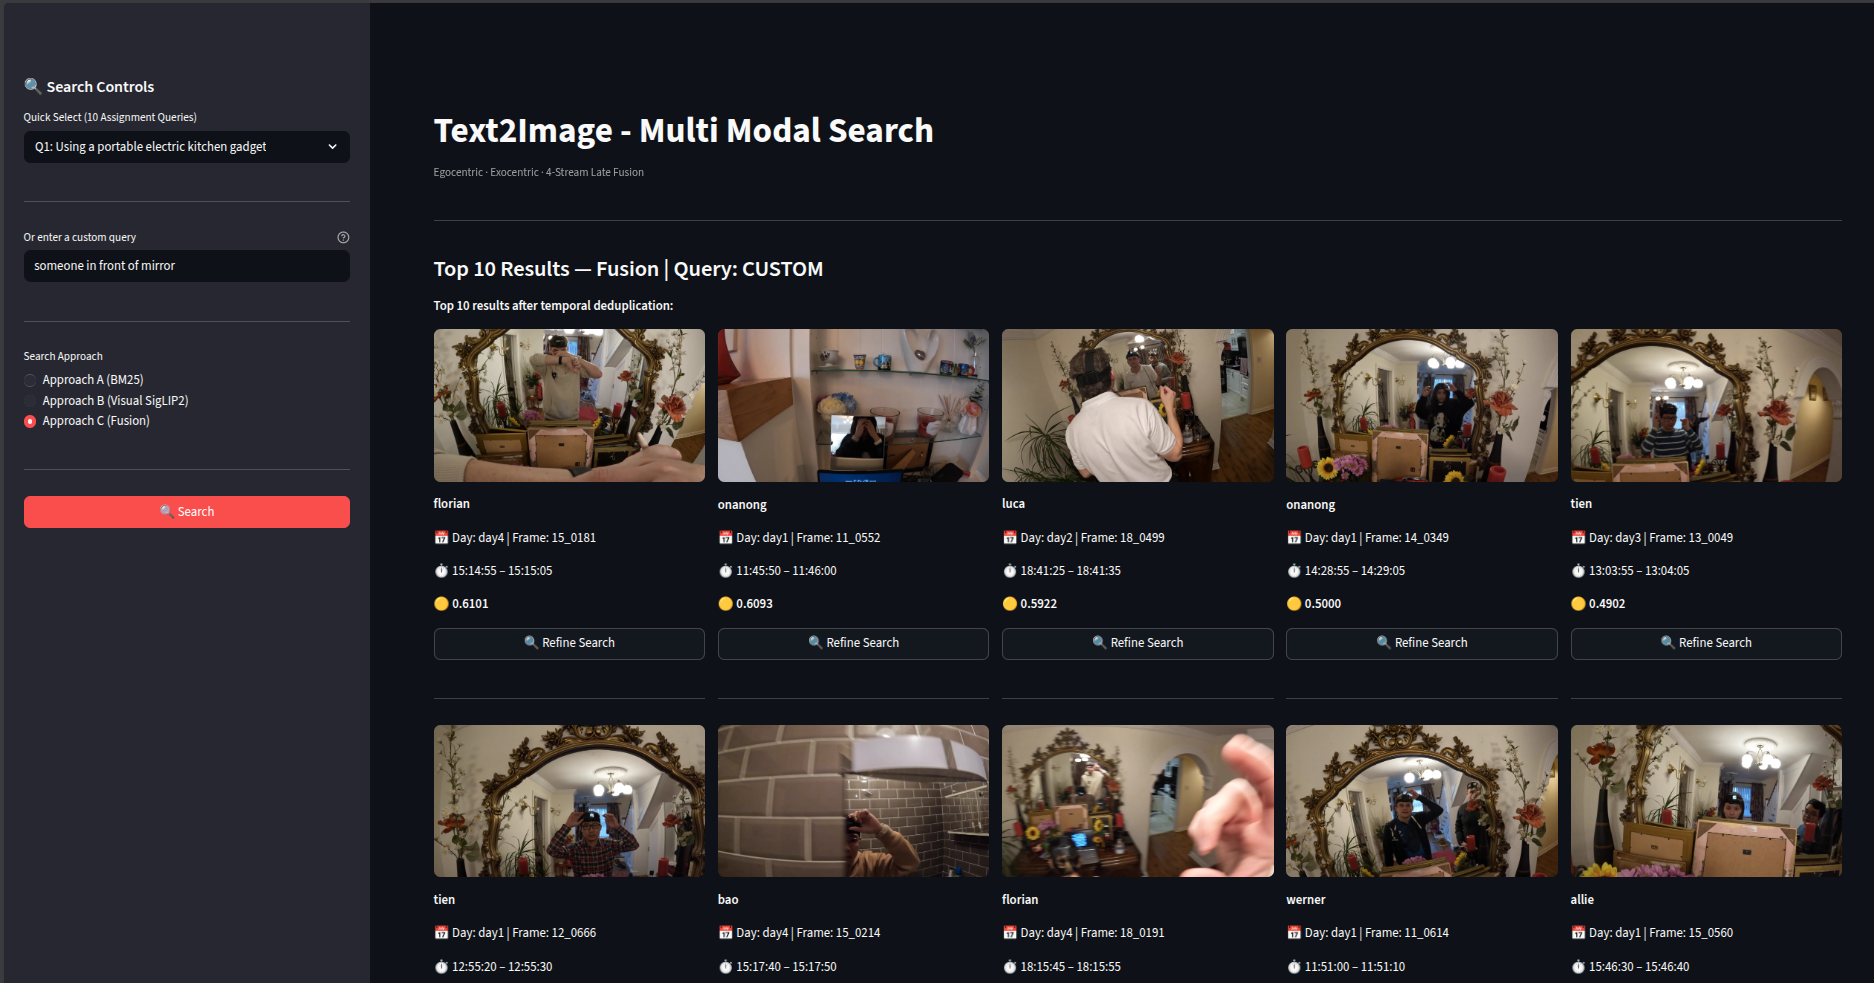
\includegraphics[width=\linewidth]{figures/streamlit_ui}
  \caption{Interactive Streamlit query interface showing top-10 retrieved frames, similarity scores, and approach selector for the MOS retrieval system.}
  \label{fig:streamlit-ui}
  \Description{Screenshot of the Streamlit search interface with query controls, approach selection, and a ranked grid of retrieved frames with scores.}
\end{figure}

\subsection{Analysis}
\label{sec:analysis}

Approach B substantially outperforms BM25 text retrieval, achieving a mean P@10 of 0.620 compared with 0.070 for Approach A. Activity queries Q4, Q5, and Q8 achieve perfect P@10 of 1.0 under Approach B, indicating that \textbf{SigLIP2} visual embeddings capture distinctive scene-level evidence more reliably than sparse transcript or caption text in this egocentric setting. This supports the central design decision of the system: when ASR is sparse or poorly aligned with frame content, dense visual embeddings become the dominant retrieval signal.

Approach C, implemented as \fusionname, ties or exceeds Approach B on 9 out of 10 queries and achieves the best overall mean P@10 of 0.640. Queries Q1 and Q9 each improve by 0.1 over the visual baseline, showing that caption and transcript evidence contributes complementary signal for activity-focused and symbol-recognition queries. No query falls below the Approach B baseline under fusion, indicating that the late-fusion and cross-encoder re-ranking stage improves precision without introducing regressions.

Approach A performs poorly as a standalone method, with a mean P@10 of 0.070 and non-zero scores only on Q1, Q2, Q6, and Q8. The limiting factor is modality mismatch: salient frame content is rarely described verbatim in co-occurring ASR transcripts, so keyword matching alone provides weak coverage for the lifelogging domain.

The OCR hallucination gate also had a measurable indexing impact. \textbf{Florence-2} hallucinated OCR text in 178,914 caption records, corresponding to 73.0\% of the 244,966-frame captioning corpus. The zero-shot \textbf{SigLIP2} cosine gate stripped all 178,914 records, yielding a 100\% removal rate. Retaining these ungrounded tokens would have injected systematic noise into both the \textbf{Whoosh} BM25 index and the \textbf{BGE-large-en-v1.5} caption embeddings, directly harming Approach A and the text component of Approach C.

\subsection{Failure Analysis}
\label{sec:failure}

Query Q7, which asks for a squirrel christmas tree ornament, remains challenging, with P@10 of 0.3 for both Approaches B and C. Global frame-level embeddings capture scene context more readily than fine-grained instance identity, so frames containing a christmas tree with multiple ornaments are compressed into a single representation that conflates several objects. A region-level grounding stage such as GroundingDINO \cite{liu2024groundingdino} would likely be necessary to localise the target ornament within cluttered scenes.

Query Q9, which asks for the ace of spades, shows a modest gain from fusion, with Approach C reaching 0.2 compared with 0.1 for Approach B. This improvement suggests that caption-derived context can help, but the query still depends on instance-level symbol recognition that remains below the semantic resolution of dense image-text embeddings trained on natural image-caption pairs.

Query Q10, which asks for a partially eaten apple, reaches only 0.1 under both Approaches B and C. The partially eaten state is a transient physical property that may produce only a weak change in a frame embedding relative to an intact apple. Detecting such state changes likely requires temporal reasoning over sequences rather than static frame-level retrieval.

\section{Conclusions}
\label{sec:conclusions}

This work shows that dense visual retrieval is the dominant signal for multimodal search over egocentric lifelogging video. \textbf{SigLIP2} achieves a mean Precision@10 of 0.620, substantially outperforming the BM25-only baseline at 0.070. The best overall effectiveness is obtained by Approach C, the \fusionname pipeline, which reaches a mean Precision@10 of 0.640. Its gains on Q1 and Q9, both improving by 0.1 over the visual baseline, show that transcript and caption evidence can provide complementary context for activity-oriented and symbol-recognition queries. Cross-encoder re-ranking with the \textbf{bge-reranker-v2-m3} model over the top-50 candidates further improves precision beyond the bi-encoder stage alone.

Several components of the system behaved as intended. The OCR hallucination gate removed 178,914 ungrounded \textbf{Florence-2} OCR-bearing caption records at a 100\% strip rate, preventing systematic noise from entering both the sparse BM25 index and the dense caption embedding space. Temporal deduplication enforced result diversity by suppressing frames within a $\pm 10$ second window of stronger results from the same stream, while cross-stream flagging exposed valid multi-angle evidence. The interactive Rocchio-style refinement mechanism also supports user feedback without rebuilding indexes.

The study also exposed clear limitations. BM25 retrieval is not sufficient as a standalone method for this domain because relevant visual content is rarely described verbatim in co-occurring ASR transcripts. Query Q7 reaches only 0.3 under both Approaches B and C because global frame-level embeddings do not resolve instance-level object identity well in cluttered scenes. Query Q10 remains at 0.1 under both approaches, suggesting that transient physical state is difficult to capture with static frame-level similarity alone.

Future work should therefore focus on richer localisation and temporal modelling. Region-level grounding methods such as \textbf{GroundingDINO} \cite{liu2024groundingdino} could help address instance-level failures such as Q7. Larger re-ranking pools may further improve precision for difficult queries. Temporal sequence modelling, as explored in \cite{lei2021less}, could support state-aware retrieval for transient object conditions such as Q10. A final direction is to replace hand-tuned fusion weights with adaptive weighting learned from relevance feedback.


\bibliographystyle{ACM-Reference-Format}
\bibliography{report}

\end{document}
